\documentclass[12pt,a4paper]{article}

% ─── Page Layout ───────────────────────────────────────────────────────────────
\usepackage[a4paper, margin=0.8in, headheight=14pt]{geometry}

% ─── Fonts (XeLaTeX) ───────────────────────────────────────────────────────────
\usepackage{fontspec}
\usepackage{unicode-math}
\setmainfont{TeX Gyre Pagella}
\setmonofont[Scale=0.88]{TeX Gyre Cursor}
\setmathfont{Latin Modern Math}

% ─── Packages ──────────────────────────────────────────────────────────────────
\usepackage{xcolor}
\usepackage{colortbl}
\usepackage{titlesec}
\usepackage{enumitem}
\usepackage{tabularx}
\usepackage{longtable}
\usepackage{booktabs}
\usepackage{array}
\usepackage{amsmath}
\usepackage{tikz}
\usetikzlibrary{shapes.geometric, arrows.meta, positioning, calc, fit, decorations.pathreplacing, patterns}
\usepackage{tcolorbox}
\tcbuselibrary{skins, breakable}
\usepackage{hyperref}
\usepackage{fancyhdr}
\usepackage{graphicx}
\usepackage{microtype}
\hyphenpenalty=10000
\exhyphenpenalty=10000
\sloppy
\usepackage{caption}
\usepackage{setspace}
\usepackage{multirow}
\usepackage{tocloft}

% ─── Q&A helper ────────────────────────────────────────────────────────────────
\newcommand{\Q}[1]{\textbf{#1}\par\noindent\ignorespaces}

% ─── Colour Palette ────────────────────────────────────────────────────────────
\definecolor{myred}{RGB}{196,30,58}
\definecolor{mydark}{RGB}{30,30,50}
\definecolor{mygreen}{RGB}{14,120,80}
\definecolor{myteal}{RGB}{0,130,140}
\definecolor{myamber}{RGB}{180,100,0}
\definecolor{mypurple}{RGB}{100,30,160}
\definecolor{mygray}{RGB}{246,247,249}
\definecolor{mgframe}{RGB}{180,185,200}
\definecolor{watermark}{RGB}{145,150,170}
\definecolor{hdrred}{RGB}{250,232,235}
\definecolor{hdrgreen}{RGB}{220,244,233}
\definecolor{hdrteal}{RGB}{220,242,244}
\definecolor{hdramber}{RGB}{253,242,215}
\definecolor{hdrpurple}{RGB}{238,228,255}
\definecolor{hdrgray}{RGB}{238,240,245}

% ─── Section Formatting ────────────────────────────────────────────────────────
\titleformat{\section}
  {\large\bfseries\color{myred}}{\thesection.}{0.5em}{}
  [\vspace{1pt}{\color{myred}\rule{\linewidth}{0.8pt}}]
\titleformat{\subsection}
  {\normalsize\bfseries\color{myteal}}{\thesubsection}{0.5em}{}
\titlespacing*{\section}{0pt}{18pt}{7pt}
\titlespacing*{\subsection}{0pt}{11pt}{4pt}

% ─── Paragraph ─────────────────────────────────────────────────────────────────
\setlength{\parindent}{0pt}
\setlength{\parskip}{4pt}

% ─── TOC Styling ───────────────────────────────────────────────────────────────
\renewcommand{\cfttoctitlefont}{\large\bfseries\color{myred}}
\renewcommand{\cftaftertoctitle}{\par\noindent{\color{myred}\rule{\linewidth}{0.8pt}}}
\setlength{\cftbeforetoctitleskip}{0pt}
\setlength{\cftaftertoctitleskip}{6pt}
\renewcommand{\cftsecfont}{\normalsize\bfseries\color{mydark}}
\renewcommand{\cftsecpagefont}{\normalsize\bfseries\color{mydark}}
\renewcommand{\cftsecleader}{\cftdotfill{\cftdotsep}}
\setlength{\cftbeforesecskip}{7pt}
\renewcommand{\cftsubsecfont}{\small\color{mydark}}
\renewcommand{\cftsubsecpagefont}{\small\color{mydark}}
\setlength{\cftbeforesubsecskip}{3pt}
\setlength{\cftsubsecindent}{1.4em}

% ─── Table helpers ─────────────────────────────────────────────────────────────
\renewcommand{\arraystretch}{1.45}
\setlength{\tabcolsep}{6pt}
\arrayrulecolor{mydark}
\newcolumntype{B}[1]{>{\small\bfseries\raggedright\arraybackslash}m{#1}}
\newcolumntype{Y}{>{\small\raggedright\arraybackslash}X}
\renewcommand{\tabularxcolumn}[1]{m{#1}}

% ─── Header / Footer ───────────────────────────────────────────────────────────
\pagestyle{fancy}
\fancyhf{}
\fancyhead[L]{\small\color{myred}\textbf{BS-B401}\;\color{mydark}--- Biology for Engineers}
\fancyhead[R]{\small\color{myteal}\textbf{Module 2 Notes}}
\fancyfoot[C]{\small\color{mydark}\thepage}
\fancyfoot[R]{\small\color{watermark}\textit{\copyright\ Biraj Sarkar (CGEC)}}
\renewcommand{\headrulewidth}{0.5pt}
\renewcommand{\footrulewidth}{0.3pt}

% ─── Hyperref ──────────────────────────────────────────────────────────────────
\hypersetup{
  colorlinks=true, linkcolor=myteal, urlcolor=myteal,
  pdfauthor={Biraj Sarkar (CGEC)},
  pdftitle={BS-B401 --- Module 2 Notes: Classification and Model Organisms}
}

% ─── tcolorbox styles ──────────────────────────────────────────────────────────
\tcbset{
  tikzbox/.style={
    colback=mygray, colframe=mgframe, boxrule=0.6pt, arc=4pt,
    left=8pt, right=8pt, top=6pt, bottom=6pt,
    colbacktitle=mgframe, coltitle=mydark, fonttitle=\small\bfseries
  },
  defbox/.style={
    colback=hdrgreen, colframe=mygreen, boxrule=0.8pt, arc=4pt,
    left=9pt, right=9pt, top=6pt, bottom=6pt,
    colbacktitle=mygreen, coltitle=white, fonttitle=\small\bfseries
  },
  formulabox/.style={
    colback=hdrteal, colframe=myteal, boxrule=0.8pt, arc=4pt,
    left=9pt, right=9pt, top=7pt, bottom=7pt,
    colbacktitle=myteal, coltitle=white, fonttitle=\small\bfseries
  },
  examplebox/.style={
    colback=hdramber, colframe=myamber, boxrule=0.8pt, arc=4pt,
    left=9pt, right=9pt, top=6pt, bottom=6pt,
    colbacktitle=myamber, coltitle=white, fonttitle=\small\bfseries
  },
  masonbox/.style={
    colback=hdrpurple, colframe=mypurple, boxrule=0.8pt, arc=4pt,
    left=9pt, right=9pt, top=6pt, bottom=6pt,
    colbacktitle=mypurple, coltitle=white, fonttitle=\small\bfseries
  },
  exambox/.style={
    colback=hdrpurple, colframe=mypurple, boxrule=1pt, arc=5pt,
    left=10pt, right=10pt, top=8pt, bottom=8pt,
    colbacktitle=mypurple, coltitle=white, fonttitle=\bfseries,
    breakable, title after break={\textbf{Frequently Asked / Viva Questions (contd.)}}
  }
}
\tcbset{breakable}
\tcbset{after={\par\color{black}}}

% ─── TikZ styles ───────────────────────────────────────────────────────────────
\tikzset{
  block/.style={rectangle, draw=myteal, fill=hdrteal,
    text width=2.4cm, align=center, minimum height=0.95cm,
    font=\small, rounded corners=3pt, line width=0.7pt},
  redblock/.style={rectangle, draw=myred, fill=hdrred,
    text width=2.4cm, align=center, minimum height=0.95cm,
    font=\small, rounded corners=3pt, line width=0.7pt},
  amberblock/.style={rectangle, draw=myamber, fill=hdramber,
    text width=2.4cm, align=center, minimum height=0.95cm,
    font=\small, rounded corners=3pt, line width=0.7pt},
  sumjunc/.style={circle, draw=myamber, fill=hdramber,
    minimum size=0.62cm, font=\small, line width=0.8pt},
  arrow/.style={-Stealth, thick, color=mydark},
  redarrow/.style={-Stealth, thick, color=myred},
  line/.style={thick, color=mydark}
}

\begin{document}

% ─── Title Page ───────────────────────────────────────────────────────────────
\begin{center}
  {\LARGE\bfseries\color{myred} BS-B401 --- Biology for Engineers}\\[5pt]
  {\normalsize\color{mydark} Semester IV \quad$\bullet$\quad 2L:1T:0P \quad$\bullet$\quad 3 Credits}\\[3pt]
  {\normalsize\color{myteal}\textbf{Module 2 Exam Notes: Classification and Model Organisms}}\\[3pt]
  {\small\color{mydark} CGEC \;$|$\; B.Tech ECE (2023--27) \;$|$\; \textit{Biraj Sarkar}}
\end{center}
\vspace{2pt}
\noindent{\color{myred}\rule{\linewidth}{1.5pt}}
\vspace{2pt}

\hypersetup{linkcolor=mydark}
\tableofcontents
\hypersetup{linkcolor=myteal}
\newpage

\section{Classification and Model Organisms}
\subsection{Levels of organisation and taxonomy}
\begin{tcolorbox}[defbox, title={Classification}]
Classification groups organisms by defined criteria. Taxonomy describes, names and classifies them. Phylogeny concerns their evolutionary relationships. A useful classification states whether the goal is to compare physical traits, ecological roles or common ancestry.
\end{tcolorbox}

\begin{itemize}[leftmargin=*, itemsep=3pt, topsep=4pt]
  \item \textbf{Biological hierarchy.} Molecules form cell components. Cells are the basic units of life. In many multicellular organisms, cells form tissues, organs and organ systems. Individuals form populations, and interacting populations form communities within ecosystems.
  \item \textbf{Taxonomic hierarchy.} Domain, kingdom, phylum, class, order, family, genus and species run from broader to narrower ranked groups. A name such as \textit{Homo sapiens} combines genus and specific epithet.
  \item \textbf{Common thread.} Cells use membranes, genetic information and basic molecular machinery such as ribosomes. Shared inherited features help connect organisms through common descent.
\end{itemize}
\par\vspace{5pt}
\begingroup
\setlength{\extrarowheight}{1pt}
\noindent\begin{tabularx}{\linewidth}{|B{3.2cm}|Y|Y|}
\hline
\textbf{Criterion} & \textbf{Question} & \textbf{Example} \\ \hline
Morphological & What are its observable form and structures? & Body plan or cell shape. \\ \hline
Biochemical & Which compounds and biochemical activities are characteristic? & Membrane lipid types or characteristic metabolic reactions. \\ \hline
Ecological & Where does it live and what ecological role does it fill? & Freshwater producer or soil decomposer. \\ \hline
Molecular & How do homologous molecules compare? & Compare ribosomal RNA sequences to infer relationships. \\ \hline
\end{tabularx}\par
\endgroup
\subsection{Cellularity and ultrastructure}
\par\vspace{5pt}
\begingroup
\setlength{\extrarowheight}{1pt}
\noindent\begin{tabularx}{\linewidth}{|B{3.1cm}|Y|Y|}
\hline
\textbf{Criterion} & \textbf{Categories} & \textbf{Key distinction} \\ \hline
Cellularity & Unicellular or multicellular & A unicellular organism carries out life functions in one cell. Multicellular forms can divide labour among specialised cells. \\ \hline
Nucleus and organelles & Prokaryote or eukaryote & Bacteria and archaea lack a membrane-bound nucleus. Eukaryotes have a nucleus and typically membrane-bound organelles. \\ \hline
Habitat & Aquatic, terrestrial and mixed & Habitat characterises where an organism lives. Some life stages use different environments. \\ \hline
\end{tabularx}\par
\endgroup
\begin{tcolorbox}[masonbox, title={Keep criteria independent}]
Yeast is unicellular and eukaryotic. A multicellular plant is also eukaryotic. The number of cells and presence of a nucleus answer different questions.
\end{tcolorbox}

\subsection{Carbon, energy and electron sources}
\par\vspace{5pt}
\begingroup
\setlength{\extrarowheight}{1pt}
\noindent\begin{tabularx}{\linewidth}{|B{3cm}|Y|Y|}
\hline
\textbf{Dimension} & \textbf{Categories} & \textbf{Meaning} \\ \hline
Carbon & Autotroph or heterotroph & Autotrophs use inorganic carbon such as carbon dioxide. Heterotrophs use preformed organic carbon. \\ \hline
Energy & Phototroph or chemotroph & Phototrophs use light. Chemotrophs obtain energy from chemical reactions. \\ \hline
Electrons & Lithotroph or organotroph & Lithotrophs use inorganic electron donors. Organotrophs use organic donors. \\ \hline
\end{tabularx}\par
\endgroup
\begin{tcolorbox}[examplebox, title={One organism can have several labels}]
An oxygenic green alga is often a photoautotroph because light supplies energy and carbon dioxide supplies carbon. In oxygenic photosynthesis, water is an inorganic electron donor. Humans are chemoorganoheterotrophs because oxidation of organic molecules supplies energy and electrons, and organic molecules supply carbon.
\end{tcolorbox}

\subsection{Nitrogen excretion}
\par\vspace{5pt}
\begingroup
\setlength{\extrarowheight}{1pt}
\noindent\begin{tabularx}{\linewidth}{|B{3.1cm}|Y|Y|}
\hline
\textbf{Group} & \textbf{Main nitrogen product} & \textbf{Typical trade-off and example} \\ \hline
Ammonotelic & Ammonia or ammonium & Highly soluble and toxic. Many aquatic bony fish can eliminate it into surrounding water. \\ \hline
Ureotelic & Urea & Less toxic than ammonia. Synthesis uses energy, but less water is needed for elimination. Example: humans. \\ \hline
Uricotelic & Uric acid & Low solubility helps save water. Production has an energy cost. Example: many birds. \\ \hline
\end{tabularx}\par
\endgroup
\section{Three Domains and Model Organisms}
\subsection{Molecular taxonomy}
\begin{tcolorbox}[defbox, title={Three-domain system}]
Ribosomal RNA comparisons helped distinguish Bacteria, Archaea and Eukarya. A domain is a rank above kingdom. The term Eucarya also appears in the original proposal. This exam framework groups life by evolutionary evidence and does not treat all prokaryotes as one clade.
\end{tcolorbox}

\begin{tcolorbox}[tikzbox, title={The three domain names}]
\centering
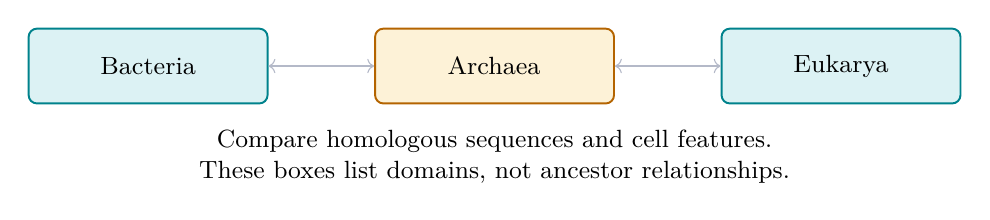
\begin{tikzpicture}[every node/.style={font=\small}]
\node[block,text width=2.8cm] (b) at (0,0) {Bacteria};
\node[amberblock,text width=2.8cm] (a) at (4.4,0) {Archaea};
\node[block,text width=2.8cm] (e) at (8.8,0) {Eukarya};
\draw[mgframe,<->] (b.east)--(a.west);
\draw[mgframe,<->] (a.east)--(e.west);
\node[align=center] at (4.4,-1.15) {Compare homologous sequences and cell features.\\These boxes list domains, not ancestor relationships.};
\end{tikzpicture}\par
\end{tcolorbox}

\textbf{Primary reading.} \href{https://pubmed.ncbi.nlm.nih.gov/2112744/}{Woese, Kandler and Wheelis (1990), three-domain proposal}.
\subsection{Six syllabus model organisms}
\par\vspace{5pt}
\begingroup
\setlength{\extrarowheight}{1pt}
\noindent\begin{tabularx}{\linewidth}{|B{4.2cm}|Y|Y|}
\hline
\textbf{Organism} & \textbf{Group} & \textbf{Why it is studied} \\ \hline
\textit{Escherichia coli} & Bacterium & Basic cell physiology and gene regulation, using well-characterised teaching and research strains. \\ \hline
\textit{Saccharomyces cerevisiae} & Budding yeast, unicellular fungus & Eukaryotic cell cycle, metabolism and genetics. \\ \hline
\textit{Drosophila melanogaster} & Fruit fly, animal & Inheritance, chromosome linkage and development. \\ \hline
\textit{Caenorhabditis elegans} & Nematode, animal & Cell lineage, development and programmed cell death. \\ \hline
\textit{Arabidopsis thaliana} & Flowering plant & Plant development, signalling and genetics. \\ \hline
\textit{Mus musculus} & House mouse, mammal & Mammalian physiology, development and inheritance. \\ \hline
\end{tabularx}\par
\endgroup
\begin{tcolorbox}[examplebox, title={Choose a model for a question}]
A researcher asking how a plant responds to light can use Arabidopsis. A question about a mammalian organ requires a different model. Model choice depends on the feature studied, available measurements and how far conclusions can be transferred.
\end{tcolorbox}

\subsection{How to classify when observable traits disagree}
\begin{enumerate}[leftmargin=*, itemsep=2pt]
  \item \textbf{Define the question.} A habitat group answers an ecological question. A group based on descent answers an evolutionary one.
  \item \textbf{Distinguish homology and convergence.} Homologous features are inherited from a common ancestor. Similar shapes can also evolve independently under similar pressures.
  \item \textbf{Use more than one kind of evidence.} Combine morphology and cellular features with comparable molecular characters. Different lines of evidence may test the same proposed relationship.
  \item \textbf{Read the branch point.} If two groups share a more recent branch point with each other than with a third group, they are closer relatives on that tree. The spacing of their names on the page is irrelevant.
\end{enumerate}

\begin{tcolorbox}[examplebox, title={Compare a whale, a fish and a land mammal}]
A whale and a fish share an aquatic habitat and a streamlined shape. A whale and a land mammal share mammalian characteristics and a more recent common ancestor. The first grouping answers where the animals live, whereas the second answers how they are related. State the criterion before defending a classification.
\end{tcolorbox}

\subsection{Explain nitrogen excretion as a water and energy trade-off}
\begin{itemize}[leftmargin=*, itemsep=2pt]
  \item \textbf{Ammonia.} Direct elimination can work where plentiful surrounding water carries soluble waste away.
  \item \textbf{Urea.} Converting nitrogen into urea costs energy, but its lower toxicity permits more concentrated elimination.
  \item \textbf{Uric acid.} Low solubility can conserve water. It also permits nitrogenous waste to accumulate in a relatively insoluble form within a shelled egg.
  \item \textbf{Qualification.} The category identifies the main excretion product under the conditions studied. The balance can change with life stage or environment.
\end{itemize}

\begin{tcolorbox}[masonbox, title={Defend a choice of model organism}]
Select a yeast for a basic eukaryotic cell-cycle question, the fruit fly or nematode for many developmental questions, Arabidopsis for plant traits, and the mouse for mammalian physiology. A shared cell mechanism can be informative across species. Whole-organism conclusions still depend on the tissue, trait and biological context.
\end{tcolorbox}

\newpage
\begin{center}
  {\large\bfseries\color{myred} Quick Revision --- Module 2}\\[3pt]
  {\small\color{mydark} Classification and Model Organisms $|$ BS-B401}
\end{center}
\noindent{\color{myred}\rule{\linewidth}{1.2pt}}\par\vspace{4pt}

\begin{tcolorbox}[formulabox, title={Key Concepts at a Glance}]
\renewcommand{\arraystretch}{1.35}
\noindent\begin{tabularx}{\linewidth}{B{4.5cm}Y}
Cell structure & Bacteria and Archaea are prokaryotic. Eukarya have a nucleus. \\[3pt]
Nutritional axes & Carbon, energy and electron source are independent dimensions. \\[3pt]
Taxonomy & Molecular comparisons add ancestry evidence to physical and ecological traits. \\[3pt]
\end{tabularx}\par
\end{tcolorbox}

\begin{tcolorbox}[defbox, title={One-Line Definitions}]
\begin{itemize}[leftmargin=*, itemsep=3pt, topsep=4pt]
  \item \textbf{Taxon.} A named group at any taxonomic rank.
  \item \textbf{Autotroph.} Organism that uses inorganic carbon as its principal carbon source.
  \item \textbf{Lithotroph.} Organism using inorganic electron donors.
\end{itemize}
\end{tcolorbox}

\begin{tcolorbox}[exambox, title={Frequently Asked / Viva Questions}]
\begin{enumerate}[topsep=0pt, label=\textbf{Q\arabic*.}, itemsep=5pt, leftmargin=*]
  \item \Q{What is the basic unit of life?}
    The cell.
  \item \Q{How does phylogeny differ from taxonomy?}
    Phylogeny deals with evolutionary relationships. Taxonomy names and classifies groups.
  \item \Q{Is every unicellular organism prokaryotic?}
    Yeast is a unicellular eukaryote.
  \item \Q{What are the three domains?}
    Bacteria, Archaea and Eukarya.
  \item \Q{Why use ribosomal RNA for comparisons?}
    Related ribosomal genes are widely shared and contain both conserved and variable features.
  \item \Q{Is lithotrophy a carbon label?}
    It describes electron donors.
  \item \Q{Which excretory product helps conserve water?}
    Uric acid.
  \item \Q{Name a plant model.}
    Arabidopsis thaliana.
  \item \Q{Name a unicellular eukaryotic model.}
    Saccharomyces cerevisiae.
  \item \Q{Why can an organism belong to several categories?}
    Each criterion describes a different feature.
\end{enumerate}
\end{tcolorbox}

\begin{tcolorbox}[tikzbox, title={Summary Comparison}]
\par\vspace{5pt}
\begingroup
\setlength{\extrarowheight}{1pt}
\noindent\begin{tabularx}{\linewidth}{|B{3.45cm}|Y|Y|}
\hline
\textbf{Criterion} & \textbf{One label} & \textbf{A distinct feature} \\ \hline
Carbon & Autotroph & Source of cell carbon. \\ \hline
Electrons & Lithotroph & Origin of electrons used in metabolism. \\ \hline
Nitrogen excretion & Ureotelic & Principal nitrogenous waste. \\ \hline
\end{tabularx}\par
\endgroup
\end{tcolorbox}

\end{document}
